\section{Reynolds stress closure}
Now let's investigate the Reynolds stress sensor, for both the continuous and the particular phase.
We first decompose the stress tensor by a sum of a spherical and deviatoric part \citep[chapter 6]{morel2015mathematical}, such as, 
\begin{equation*}
    \cavg{\textbf{u'u'}}
    = \frac{2}{3}\cavg{T}\left(
        \textbf{I}
        + \cavg{\textbf{B}}
    \right),
\end{equation*}
where we introduced the turbulent kinetic energy, $\cavg{T} = \frac{1}{2}\cavg{\textbf{u'u'}}:\textbf{I}$ and the deviatoric part of the Reynolds stress as, 
$\cavg{\textbf{B}} = \cavg{\textbf{u'u'}}/(2\cavg{T}) - \frac{1}{3}$.
A similar logic can be applied to the particular averaged Reynolds stress yielding, 
$
\pnavg{\textbf{u}'_\alpha \textbf{u}_\alpha'}
    = \frac{2}{3}\pnavg{T_\alpha}\left(
        \textbf{I}
        + \pnavg{\textbf{B}_\alpha}
    \right)
$.
In this case $\pnavg{T_\alpha}$ is the granular temperature from kinetic theory \citep{rao2008introduction}. 
Notice that the non-diagonal components of $\cavg{\textbf{B}}$ and  $\pnavg{\textbf{B}_\alpha}$ are all null due to the symmetry of the model. 
Therefore, they will not be shown here. 
\subsection{The continuous phase Reynolds stress}
The fluid averaged kinetic energy can be easily scaled on the numerical results shown \ref{fig:Tf_Bf}(left).
Indeed, we found out that 
\begin{equation}
    \frac{\cavg{T}}{U^2} \approx \frac{\phi}{Ga^2}5.98\cdot10^{4} ,
    \label{eq:Tf_scaling}
\end{equation}
where we use the drift velocity $U$ to make $T$ dimensionless. 
\begin{figure}[h!]
    \centering
    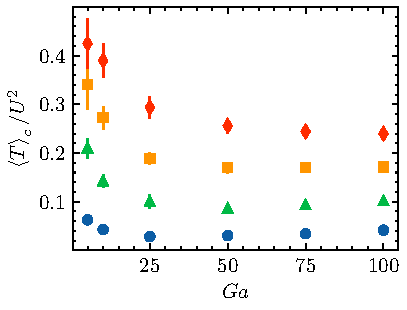
\includegraphics[height=0.3\textwidth]{image/HOMOGENEOUS/fCA/Tf.pdf}
    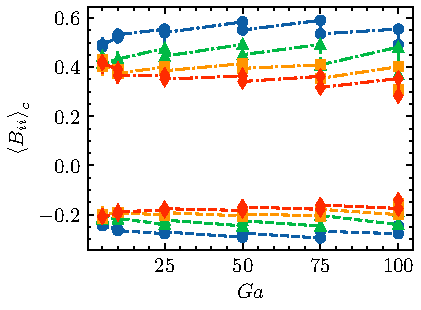
\includegraphics[height=0.3\textwidth]{image/HOMOGENEOUS/fCA/Bf.pdf}
    \caption{(left) Dimensionless turbulent kinetic energy in terms of the \textit{Galileo} number for different $\phi$. (dots) Numerical simulations, (dashed line) empirical formula \ref{eq:Tf_scaling}.
    (right) deviatoric part of the Reynolds stress, ($\bullet$) are the vertical components, $B_{yy}$, ($\blacktriangle$) are the horizontal components, $B_{xx} = B_{zz}$.}
    \label{fig:Tf_Bf}
\end{figure}
In opposition to the drift velocity, the dimensionless turbulent kinetic energy scale as $\sim \phi$ regardless of the \textit{Galileo} number. 
As shown previously $U \sim \phi^{1/3}$, consequently the turbulent kinetic energy scale as $\cavg{T} \sim \phi^{5/3}$. 
Besides, $\cavg{T}$ is a monotonic function of $Ga$ with a growth rate of $0.91$. 
Regarding the deviatoric part of the Reynolds stress tensor, namely, $\cavg{\textbf{B}}$, it can be approximated by, roughly, $\cavg{\textbf{B}_{yy}} \approx 0.4$ and $\cavg{\textbf{B}_{zz}} = \cavg{\textbf{B}_{xx}}  \approx - 0.2$.
Therefore, the \textit{Reynolds} stress is clearly oriented, indeed the stress is greater in the direction of the flow. 
Also, as depicted by \ref{fig:Tf_Bf} (right), at high $Ga$ and $\phi$ those components slightly tend to lower values, whether it is for the horizontal or vertical components. 
This means that the global Reynolds stress tends to be isotropic with for high $Ga$ and $\phi$. 
In \citet{jackson2000dynamics} they stipulate that at high rate of collision the \textit{Reynolds} stress tends to be isotropic. 
Which is in accordance with our findings since, $Ga$ and $\phi$ are directly correlated to the rate of collision. 
For now a good approximation of $\cavg{\textbf{B}}$ is 
\begin{equation}
    \cavg{\textbf{B}} 
    \approx 0.4 \textbf{dd} + 0.2 (\textbf{I} - \textbf{dd}),
    \label{eq:Bf_scaling}
\end{equation}
where $\textbf{d}$ is the unit vector following the direction of the flow, in our case, $\textbf{d} = \textbf{g}/g$ or more generally, $\textbf{d} = U/|U|$. 

\subsection{The particular phase Reynolds stress}
Now let's focus on the particular averaged Reynolds stress tensor.
\ref{fig:Talpha_Balpha} shows that the granular temperature behavior is quite similar from the continuous averaged turbulent kinetic energy.
\begin{figure}[h!]
    \centering
    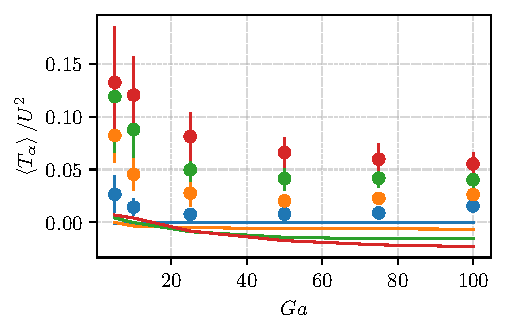
\includegraphics[height=0.3\textwidth]{image/HOMOGENEOUS/fPA/Talpha.pdf}
    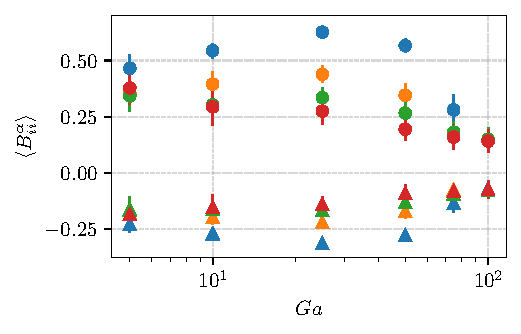
\includegraphics[height=0.3\textwidth]{image/HOMOGENEOUS/fPA/Bf.pdf}
    \caption{(left) Dimensionless turbulent kinetic energy in terms of the \textit{Galileo} number for different $\phi$. (dots) Numerical simulations, (dashed line) empirical formula \ref{eq:Talpha_scaling}.
    (right) deviatoric part of the Reynolds stress, ($\bullet$) are the vertical components, $B_{yy}$, ($\blacktriangle$) are the horizontal components, $B_{xx} = B_{zz}$.}
    \label{fig:Talpha_Balpha}
\end{figure}
We can also provide a scaling for the granular temperature, it reads as,  
\begin{equation}
    \frac{\pnavg{T_\alpha}}{U^2}  \approx \frac{\phi}{Ga^2} 2.86\cdot10^{4} 
    \label{eq:Talpha_scaling}
\end{equation}
From \ref{fig:Talpha_Balpha} we observe that this scaling is valid for the lowest \textit{Galileo}. 
The deviatoric part of $\pnavg{T_\alpha}$ is displayed on \ref{fig:Talpha_Balpha}.
It tells us that the Reynolds stress for the particular phase tends to be isotropic in the same way as $\cavg{T}$. 
Indeed, the components of $\pnavg{\textbf{B}}$ go to zero with increasing $Ga$ and $\phi$. 
This behavior is explained by the higher rate of collision present for higher volume fraction and inertia \citep[chapter 1]{jackson2000dynamics}